\subsection{Inverse Dynamics and Control Simulations}\label{S04-4}

Dada a lei de controle apresentada na sub-se\c{c}\~ao 2.4 e o modelo din\^amico apresentado na sub-se\c{c}\~ao anterior, nesta sub-se\c{c}\~ao realizaremos simula\c{c}\~oes da din\^amica inversa e da aplica\c{c}\~ao da lei de controle no mecanismo 5R balanceado e desbalancedo. Para tanto, \'e necess\'ario definir valores para os par\^ametros do mecanismos, as condi\c{c}\~oes iniciais do sistema, trajetórias de referência e os par\^ametros do controlador.

Assim, definimos:

\begin{itemize}
\item Par\^ametros físicos fixos dos mecanismos RR utilizados para formar o 5R:

\begin{itemize}
\begin{multicols}{2}
\item $a_{1,1} = 0.1 \, m$
\item $a_{1,2} = 0.2 \, m$
\item $m_{1, \llB_1} = 0.2 \, kg$
\item $m_{1, \llB_2} = 0.4 \, kg$
\item $m_{2, \llB_1} = 1.5 \, kg$
\item $I_{1, \llB_1} = 67 \cdot 10^{-5} \, kg \, m^2$
\item $I_{1, \llB_2} = 134 \cdot 10^{-5} \, kg \, m^2$
\item $\gamma_{1, \llB_1} = \gamma_{1, \llB_2} = 0.5$
\end{multicols}
\end{itemize}

\item Par\^ametros físicos ajustáveis dos RR balanceados:

\begin{itemize}
\begin{multicols}{2}
\item $\gamma_{3, \llB_1} = 3.0$
\item $\gamma_{4, \llB_1} = 1.7$
\item $m_{3, \llB_1} = m_{4, \llB_1} = 1.0 \, kg$ 
\end{multicols}
\end{itemize}

\item Par\^ametros físicos ajustáveis dos RR desbalanceados:

\begin{itemize}
\item $m_{3, \llB_1} = m_{4, \llB_1} = 0$
\end{itemize}


\item Posicionamento das bases dos mecanismos RR para formar o 5R:

\begin{itemize}
\begin{multicols}{2}
\item $q_{1,\ttp_1,1} = -0.1 \, m$
\item $q_{1,\ttp_1,2} = 0 $
\item $q_{2,\ttp_1,1} = 0.1 \, m$
\item $q_{2,\ttp_1,2} = 0 $
\end{multicols}
\end{itemize}

\item Par\^ametros do controlador utilizado:

\begin{itemize}
\begin{multicols}{2}
\item $\lambda = 40$
\item $k = 10$
\end{multicols}
\end{itemize}

\item Condi\c{c}\~oes iniciais de posi\c{c}\~ao para o mecanismo 5R:

$$\begin{cases}
q_{1,\ttp_3,1}(0) = q_{2,\ttp_3,1}(0) = 0 \\
q_{1,\ttp_3,2}(0) = q_{2,\ttp_3,2}(0) = 0.02 \,m \\
q_{3, \llR_3}(0) = 173.282^\circ \\
q_{1,\llR_1}(0) = 175.249^\circ \\
q_{1,\llR_2}(0) = 188.11^\circ \\
q_{2,\llR_1}(0) = 4.75078^\circ \\
q_{2,\llR_2}(0) = 171.89^\circ \\
\end{cases}$$

\item Trajet\'oria de refer\^encia 1:

$$ \begin{cases}
q_{1,\ttp_3,1}^\sdia(t) = q_{2,\ttp_3,1}^\sdia(t) = 0 \\
q_{1,\ttp_3,2}^\sdia(t) = q_{2,\ttp_3,2}^\sdia(t) = 0.02 + 0.22 \Big( \frac{t}{5} - \frac{1}{2\pi} \sin \big( \frac{2\pi t}{5} \big) \Big) \\
\end{cases}$$

\item Trajet\'oria de refer\^encia 2:

$$ \begin{cases}
q_{1,\ttp_3,1}^\sdia(t) = q_{2,\ttp_3,1}^\sdia(t) = 0.005 \sin(7t) \\
q_{1,\ttp_3,2}^\sdia(t) = q_{2,\ttp_3,2}^\sdia(t) = 0.14 - 0.12 \cos(7t) \\
\end{cases}$$

\end{itemize}

Foram explicitadas apenas algumas coordenadas das trajet\'orias de refer\^encia, pois, definindo estas, as outras podem ser encontradas num\'erica ou analiticamente utilizando os v\'inculos de posi\c{c}\~ao e a condi\c{c}\~ao de montagem do mecanismo.

Para as simula\c{c}\~oes da lei de controle, a fun\c{c}\~ao $y(x) = \sign(x)$ foi substituida pela fun\c{c}\~ao $y_{sat}(x) = \frac{2}{\pi}\arctan(159.1 x)$, a qual apresenta as seguintes propriedades: $y_{sat}(0.2) = -y_{sat}(0.2) = 0.98$ e $y_{sat}(\infty) = - y_{sat}(-\infty) = 1$. Sua utiliza\c{c}\~ao torna muito mais eficiente as simula\c{c}\~oes num\'ericas, evita o chattering nos atuadores e ainda garante um erro em regime permanente desprez\'ivel para esta aplica\c{c}\~ao.

\begin{figure}[H]
	\centering
	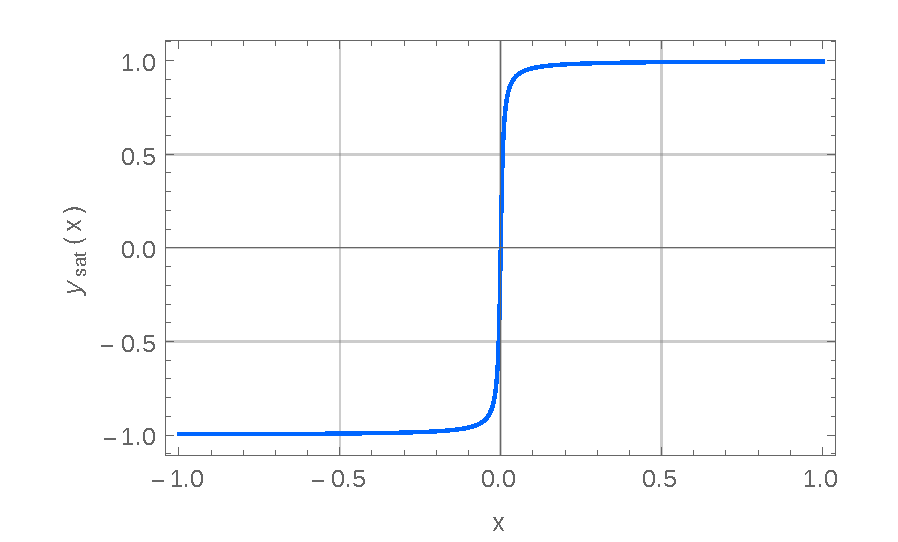
\includegraphics[scale=0.5]{Sat.pdf}
	\caption{Fun\c{c}\~ao de satura\c{c}\~ao}
	\label{Sat}
\end{figure}

Na simula\c{c}\~oes da din\^amica inversa, calculam-se os esfor\c{c}os dos atuadores necess\'arios para que o mecanismo siga exatamente a traje\'oria de refer\^encia, ignorando as condi\c{c}\~oes iniciais de velocidade que ser\~ao definidas.

\begin{itemize}
\item[A)] Simula\c{c}\~ao da trajet\'oria 1: \\

Na simula\c{c}\~ao lei de controle sup\~oe-se as seguintes condi\c{c}\~oes iniciais de velocidades:

$$\begin{cases}
\dot{q}_{1,\ttp_3,1}(0) = \dot{q}_{2,\ttp_3,1}(0) = 0 \\
\dot{q}_{1,\ttp_3,2}(0) = \dot{q}_{2,\ttp_3,2}(0) = 1 \,m/s \\
\dot{q}_{3, \llR_3}(0) = -5.871 rad/s \\
\dot{q}_{1,\llR_1}(0) = -4.153 rad/s \\
\dot{q}_{1,\llR_2}(0) = 7.089 rad/s \\
\dot{q}_{2,\llR_1}(0) = 4.153 rad/s \\
\dot{q}_{2,\llR_2}(0) = -7.089 rad/s \\
\end{cases}$$

Isso faz com que haja um erro de velocidade n\~ao nulo para $t=0$ e torna mais interessante a anal\'ise da din\^amica dos erros de posi\c{c}\~ao e velocidade.

Aqui seguem os gr\'aficos da trajet\'oria de refer\^encia 1 para algumas coordenadas:

\begin{figure}[ht]
\centering
\begin{minipage}[b]{0.45\linewidth}
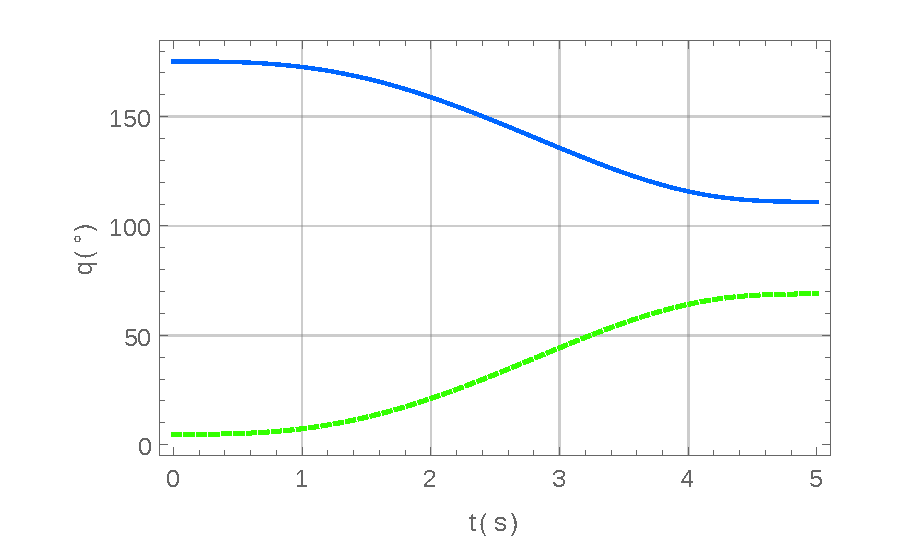
\includegraphics[scale=0.5]{AnglesA.pdf}
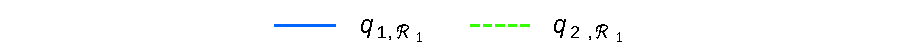
\includegraphics[scale=0.5]{AnglesAsub.pdf}
\label{fig:AnglesA}
\end{minipage}
\quad
\begin{minipage}[b]{0.45\linewidth}
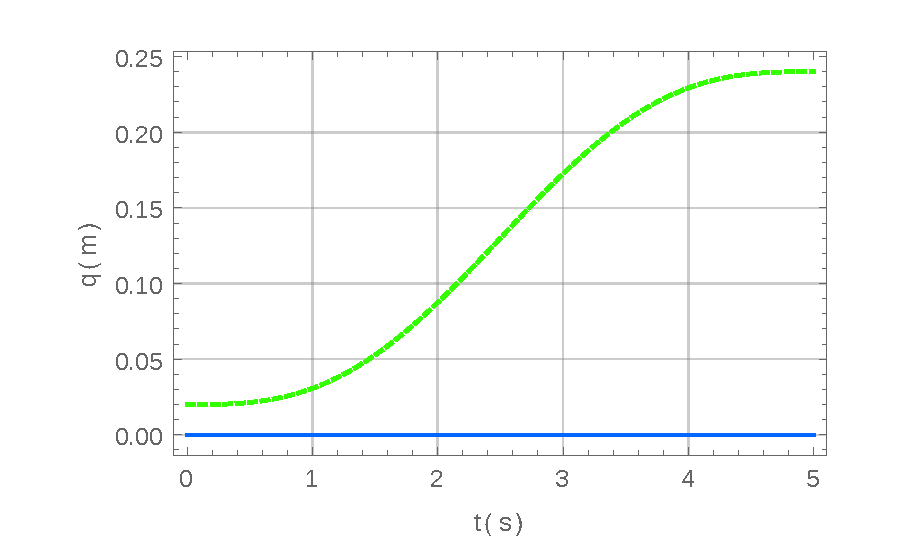
\includegraphics[scale=0.5]{XA.pdf}
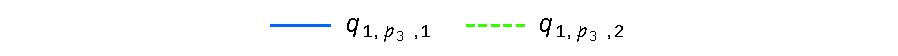
\includegraphics[scale=0.5]{XAsub.pdf}
\label{fig:XA}
\end{minipage}
\caption{Trajet\'oria de refer\^encia 1}
\end{figure}

\begin{itemize}
\item[A.1)] Mecanismo balanceado \\

Simula\c{c}\~ao dos esfor\c{c}os aplicados pelos atuadores:

\begin{figure}[H]
\centering
\begin{minipage}[b]{0.45\linewidth}
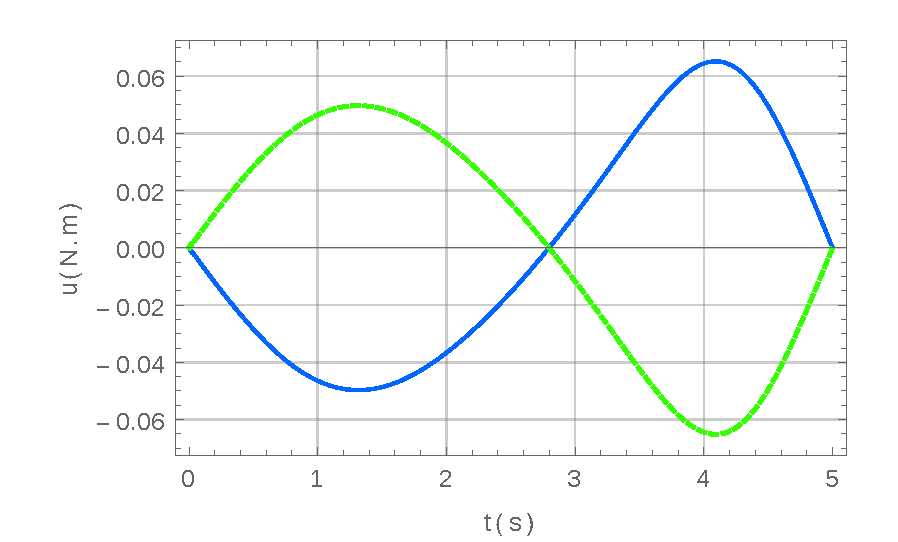
\includegraphics[scale=0.5]{InverseDynamicsA1.pdf}
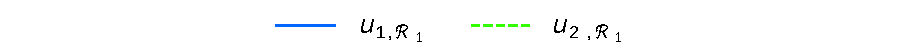
\includegraphics[scale=0.5]{InverseDynamicsA1sub.pdf}
\label{fig:InverseDynamicsA1}
\caption{Inverse dynamics simulation}
\end{minipage}
\quad
\begin{minipage}[b]{0.45\linewidth}
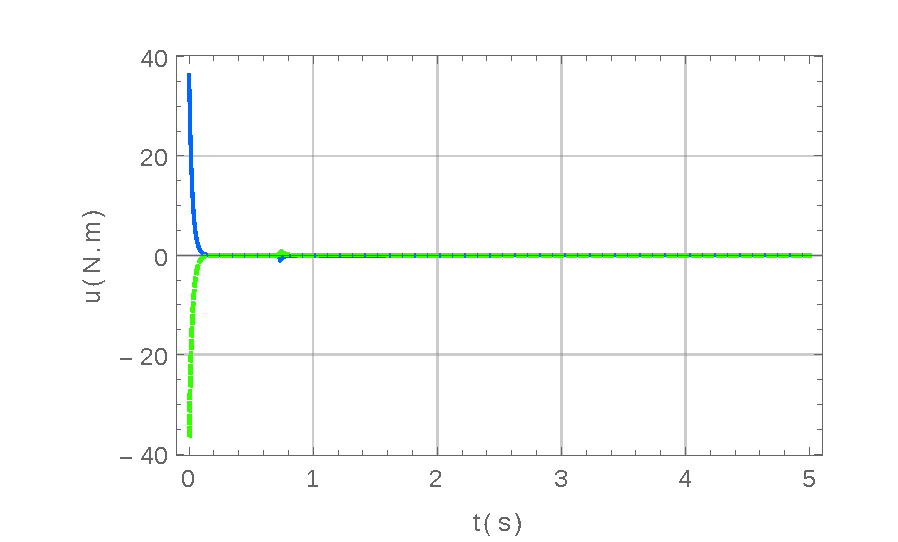
\includegraphics[scale=0.5]{ControlA1.pdf}
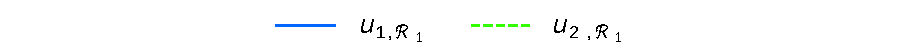
\includegraphics[scale=0.5]{ControlA1sub.pdf}
\label{fig:ControlA1}
\caption{Control inputs}
\end{minipage}
\end{figure}

Din\^amica do erro de controle:

\begin{figure}[H]
\centering
\subfigure[Position error norm]{%
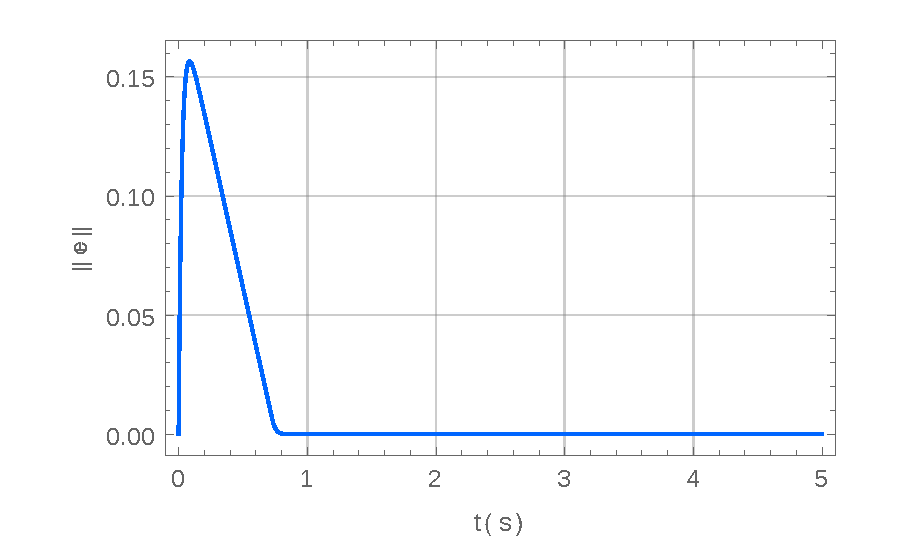
\includegraphics[scale=0.37]{PositionErrorA1.pdf}
\label{fig:PositionErrorA1}}
\quad
\subfigure[Velocity error norm]{%
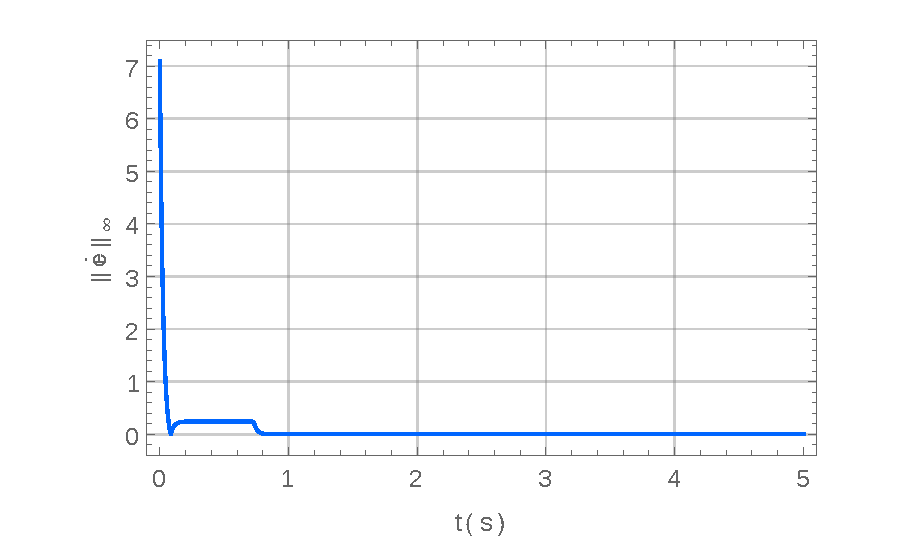
\includegraphics[scale=0.37]{VelocityErrorA1.pdf}
\label{fig:VelocityErrorA1}}
\subfigure[$||\ms|| = || \dot{\me} + \lambda \me ||$]{%
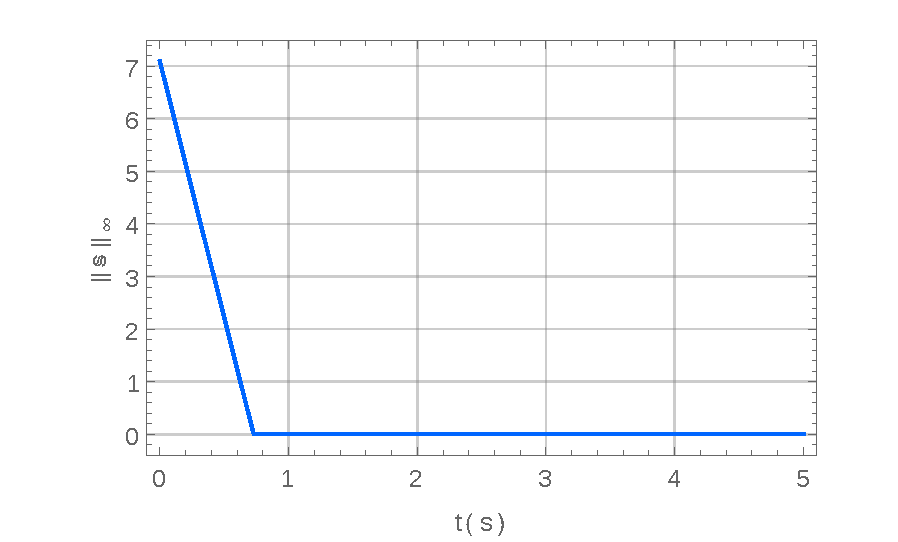
\includegraphics[scale=0.37]{sA1.pdf}
\label{fig:sA1}}
%
\caption{Error dynamics}
\label{fig:figure}
\end{figure}

\item[A.2)] Mecanismo desbalanceado \\

Simula\c{c}\~ao dos esfor\c{c}os aplicados pelos atuadores:

\begin{figure}[H]
\centering
\begin{minipage}[b]{0.45\linewidth}
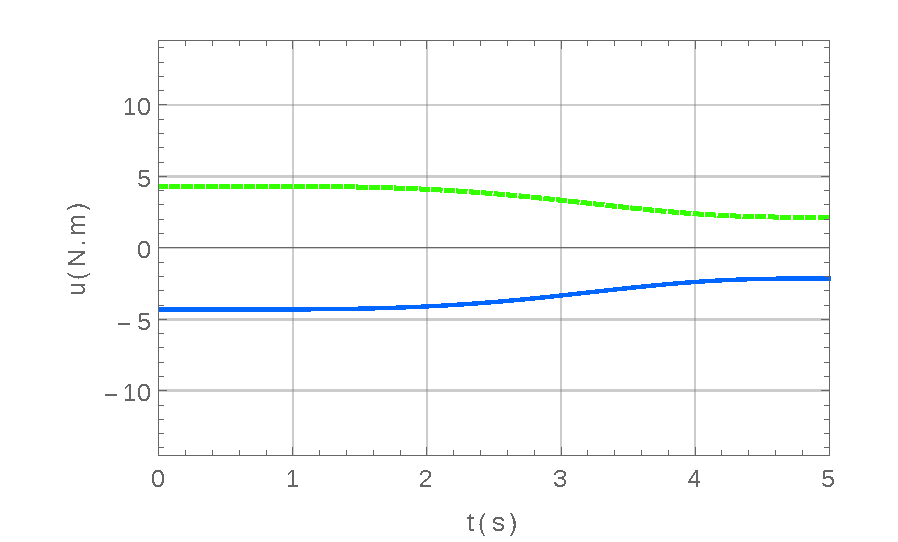
\includegraphics[scale=0.5]{InverseDynamicsA2.pdf}
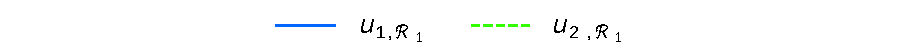
\includegraphics[scale=0.5]{InverseDynamicsA1sub.pdf}
\label{fig:InverseDynamicsA2}
\caption{Inverse dynamics simulation}
\end{minipage}
\quad
\begin{minipage}[b]{0.45\linewidth}
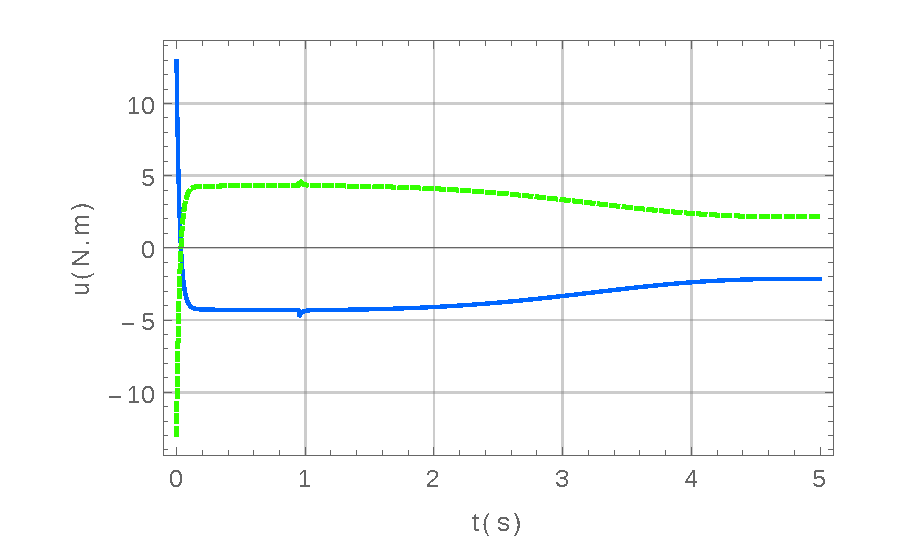
\includegraphics[scale=0.5]{ControlA2.pdf}
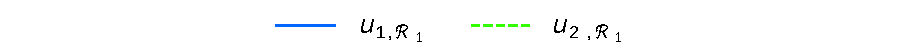
\includegraphics[scale=0.5]{ControlA1sub.pdf}
\label{fig:ControlA2}
\caption{Control inputs}
\end{minipage}
\end{figure}

Din\^amica do erro de controle:

\begin{figure}[H]
\centering
\subfigure[Position error norm]{%
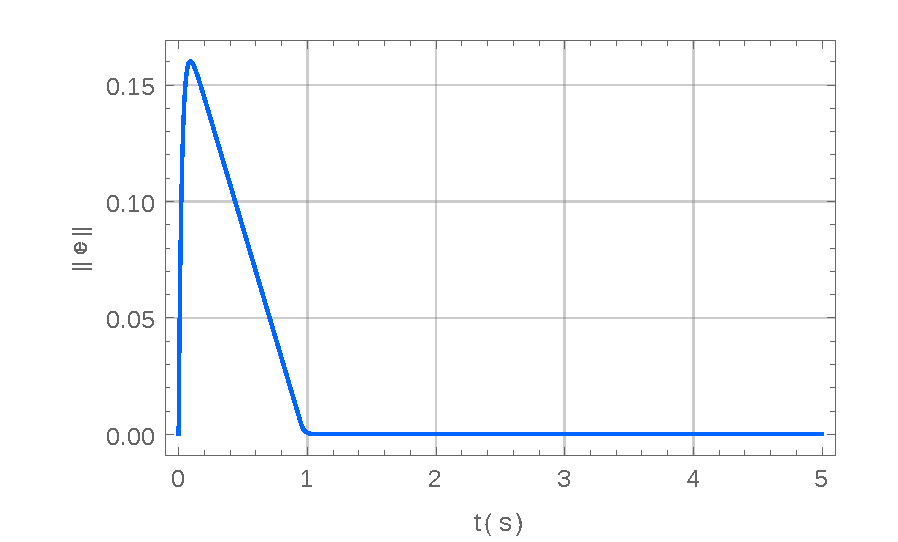
\includegraphics[scale=0.37]{PositionErrorA2.pdf}
\label{fig:PositionErrorA2}}
\quad
\subfigure[Velocity error norm]{%
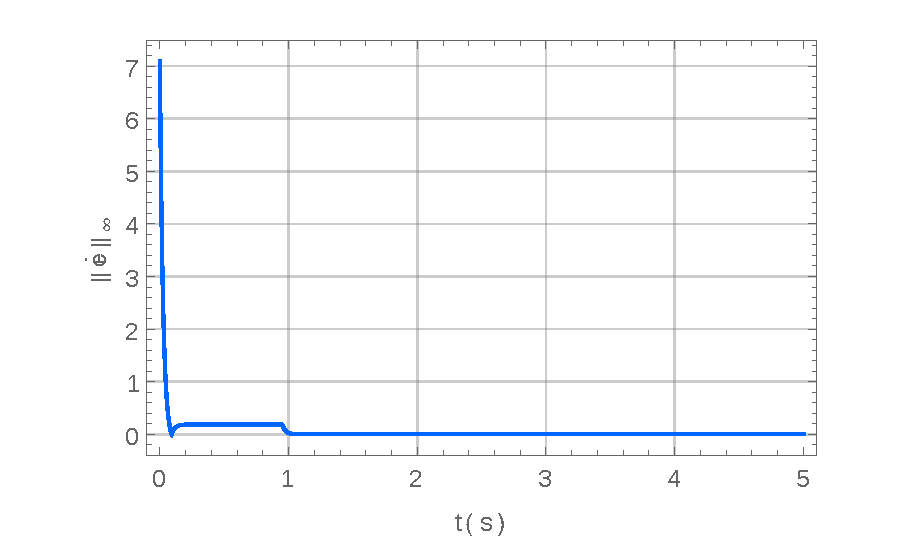
\includegraphics[scale=0.37]{VelocityErrorA2.pdf}
\label{fig:VelocityErrorA2}}
\subfigure[$||\ms|| = || \dot{\me} + \lambda \me ||$]{%
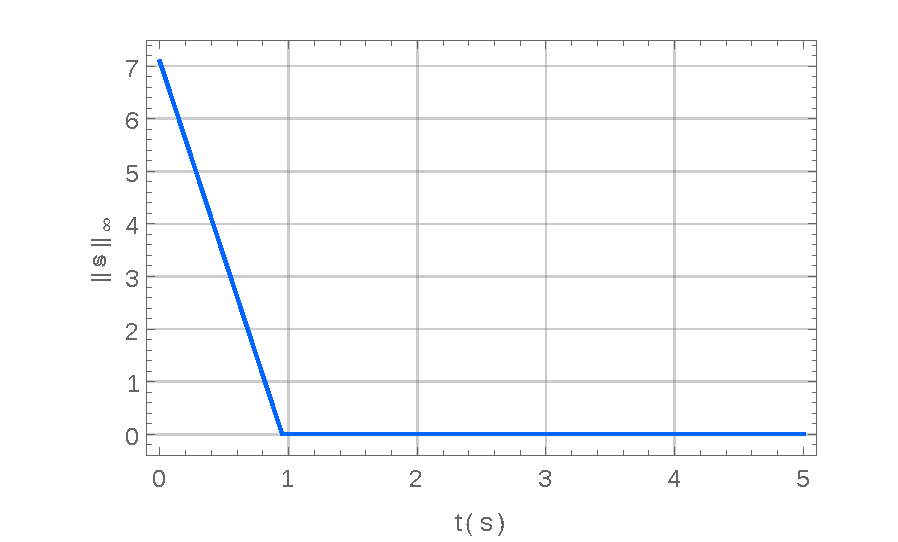
\includegraphics[scale=0.37]{sA2.pdf}
\label{fig:sA2}}
%
\caption{Error dynamics}
\label{fig:figure}
\end{figure}


\end{itemize}

Pode-se observar que, na maior parte do tempo, os esfor\c{c}os realizados pelos atuadores no caso do mecanismo desbalanceado s\~ao bem maiores do que no caso do mecanismo balanceado. Esse resultado \'e esperado, pois a trajet\'oria de refer\^encia 1 \'e um movimento lento, o que significa que a contrubui\c{c}\~ao do peso deve ser mais significativa do que a contribui\c{c}\~ao das for\c{c}as de in\'ercia nos esfor\c{c}os dos atuadores.


\item[B)] Simula\c{c}\~ao da trajet\'oria 2: \\

Na simula\c{c}\~ao lei de controle sup\~oe-se condi\c{c}\~oes iniciais de velocidades nulas.

Aqui seguem os gr\'aficos da trajet\'oria de refer\^encia 2 para algumas coordenadas:

\begin{figure}[ht]
\centering
\begin{minipage}[b]{0.45\linewidth}
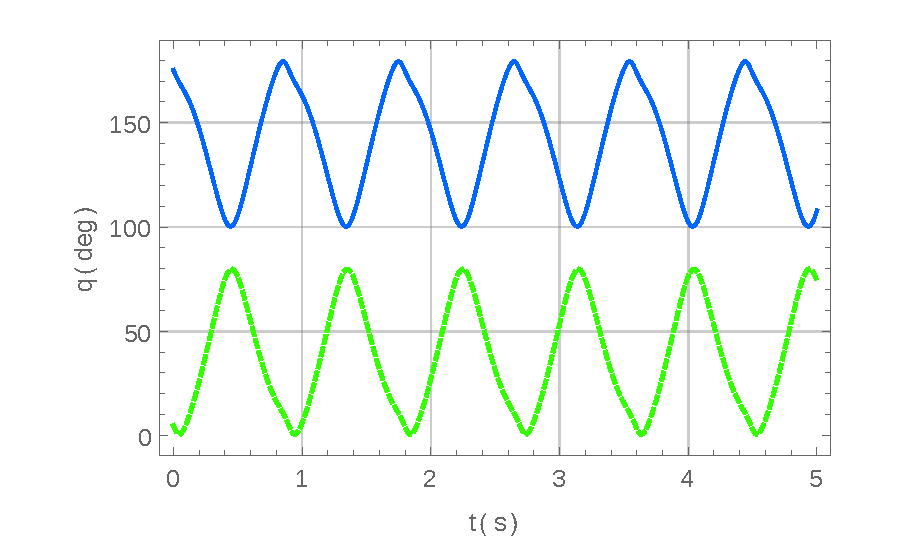
\includegraphics[scale=0.5]{AnglesB.pdf}
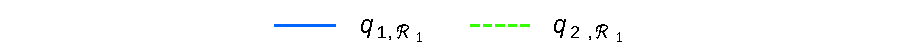
\includegraphics[scale=0.5]{AnglesAsub.pdf}
\label{fig:AnglesB}
\end{minipage}
\quad
\begin{minipage}[b]{0.45\linewidth}
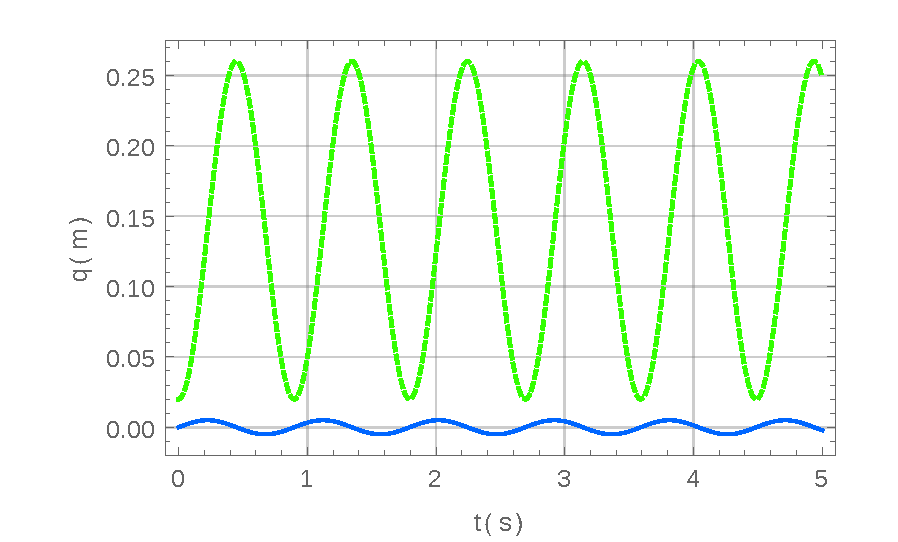
\includegraphics[scale=0.5]{XB.pdf}
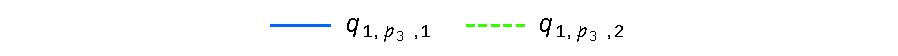
\includegraphics[scale=0.5]{XAsub.pdf}
\label{fig:XB}
\end{minipage}
\caption{Trajet\'oria de refer\^encia 1}
\end{figure}

\begin{itemize}
\item[B.1)] Mecanismo balanceado \\

Simula\c{c}\~ao dos esfor\c{c}os aplicados pelos atuadores:

\begin{figure}[H]
\centering
\begin{minipage}[b]{0.45\linewidth}
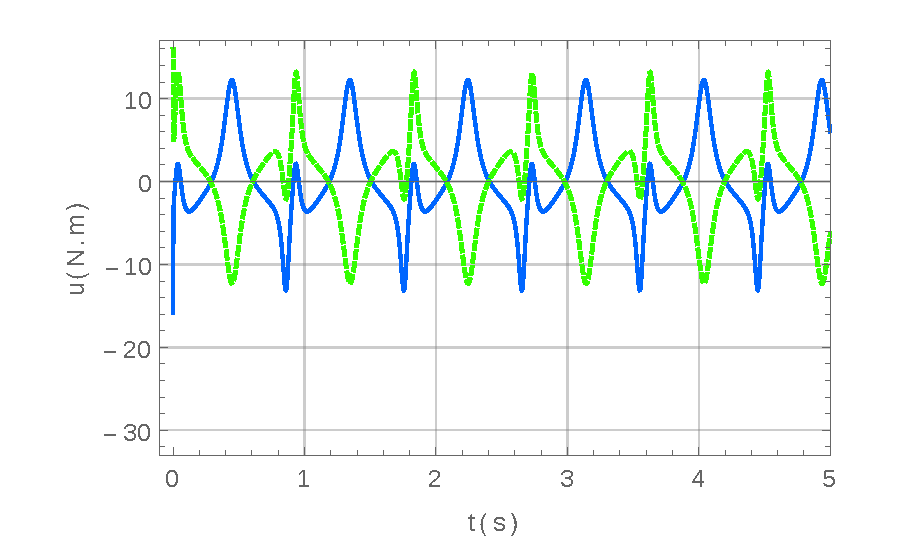
\includegraphics[scale=0.5]{InverseDynamicsB1.pdf}
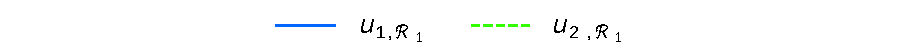
\includegraphics[scale=0.5]{InverseDynamicsA1sub.pdf}
\label{fig:InverseDynamicsB1}
\caption{Inverse dynamics simulation}
\end{minipage}
\quad
\begin{minipage}[b]{0.45\linewidth}
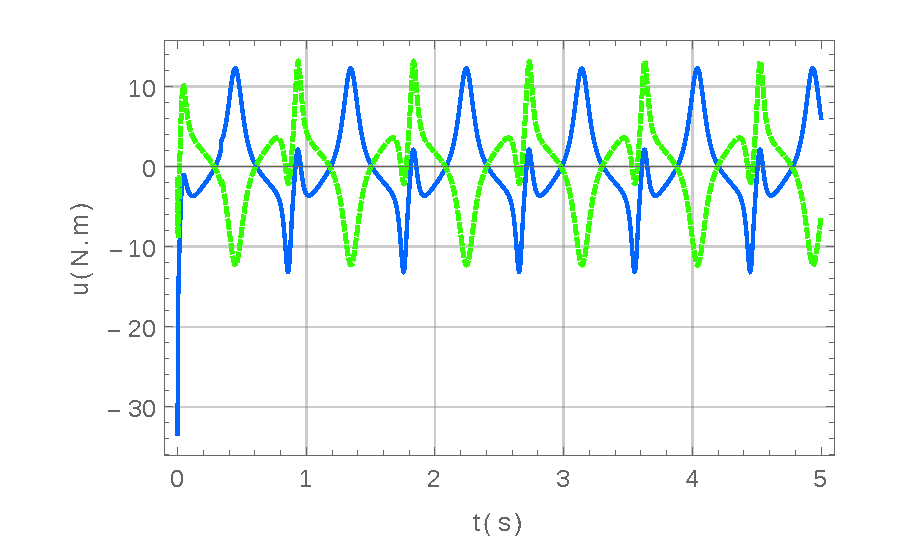
\includegraphics[scale=0.5]{ControlB1.pdf}
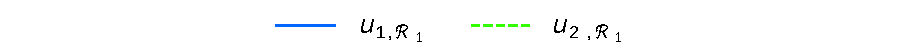
\includegraphics[scale=0.5]{ControlA1sub.pdf}
\label{fig:ControlB1}
\caption{Control inputs}
\end{minipage}
\end{figure}

Din\^amica do erro de controle:

\begin{figure}[H]
\centering
\subfigure[Position error norm]{%
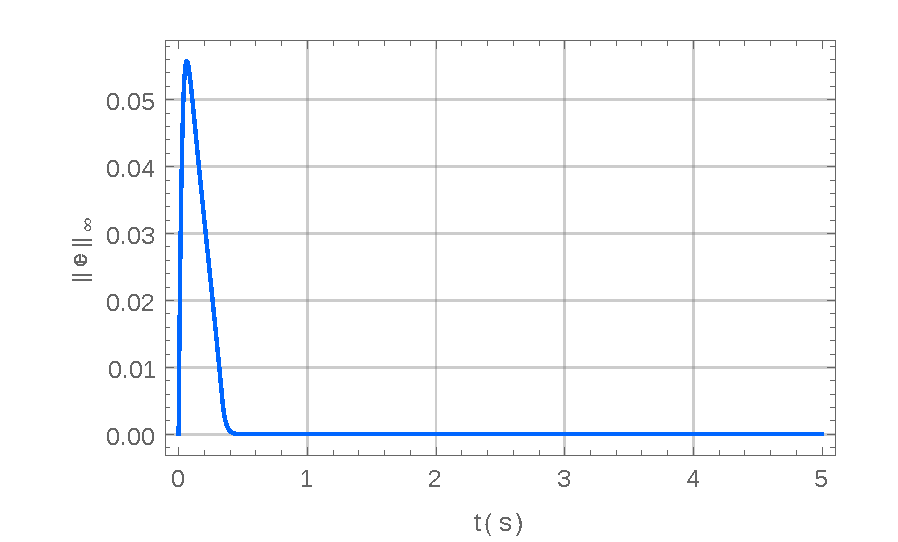
\includegraphics[scale=0.37]{PositionErrorB1.pdf}
\label{fig:PositionErrorB1}}
\quad
\subfigure[Velocity error norm]{%
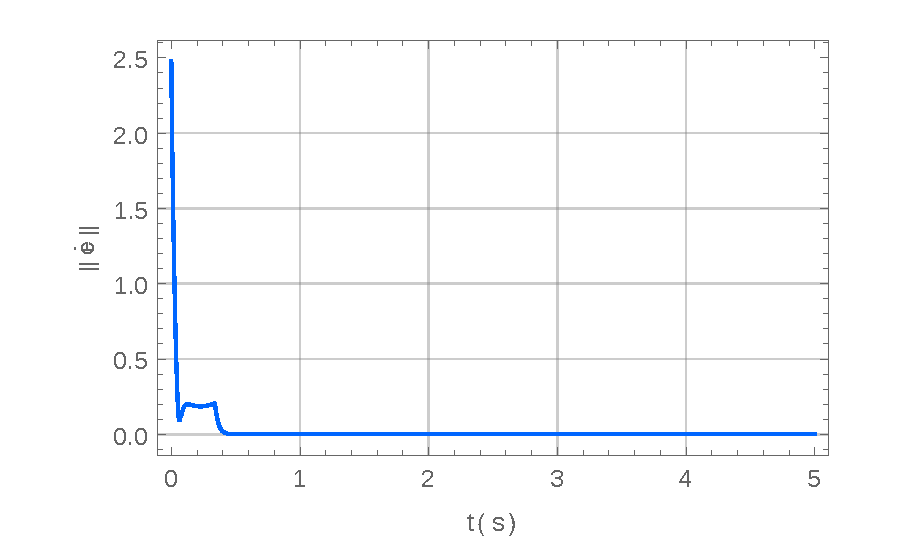
\includegraphics[scale=0.37]{VelocityErrorB1.pdf}
\label{fig:VelocityErrorB1}}
\subfigure[$||\ms|| = || \dot{\me} + \lambda \me ||$]{%
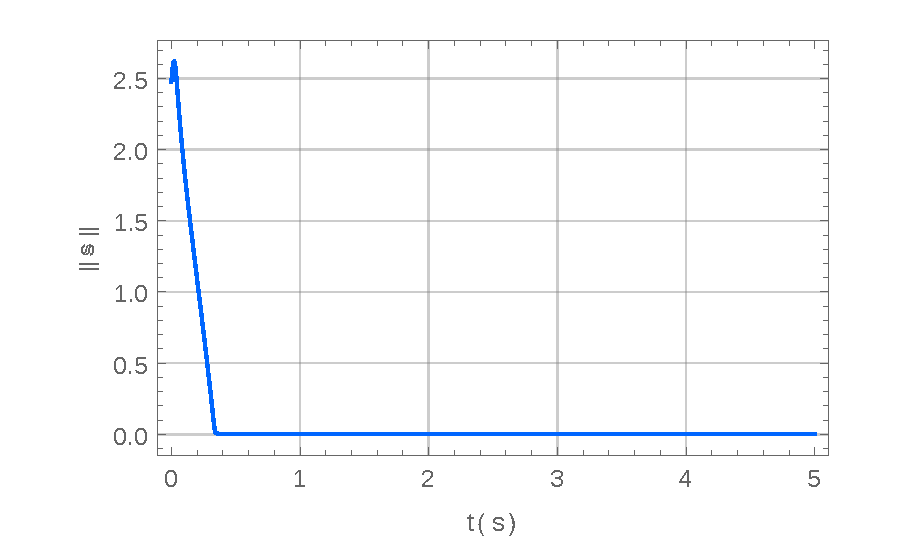
\includegraphics[scale=0.37]{sB1.pdf}
\label{fig:sA1}}
%
\caption{Error dynamics}
\label{fig:figure}
\end{figure}

\item[B.2)] Mecanismo desbalanceado \\

Simula\c{c}\~ao dos esfor\c{c}os aplicados pelos atuadores:

\begin{figure}[H]
\centering
\begin{minipage}[b]{0.45\linewidth}
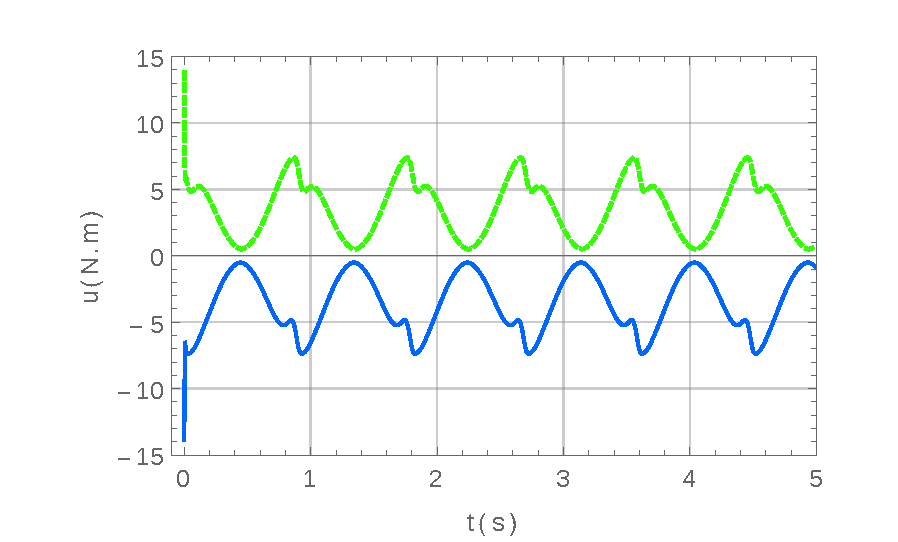
\includegraphics[scale=0.5]{InverseDynamicsB2.pdf}
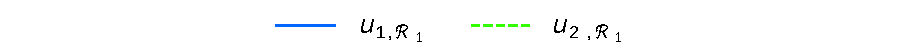
\includegraphics[scale=0.5]{InverseDynamicsA1sub.pdf}
\label{fig:InverseDynamicsB2}
\caption{Inverse dynamics simulation}
\end{minipage}
\quad
\begin{minipage}[b]{0.45\linewidth}
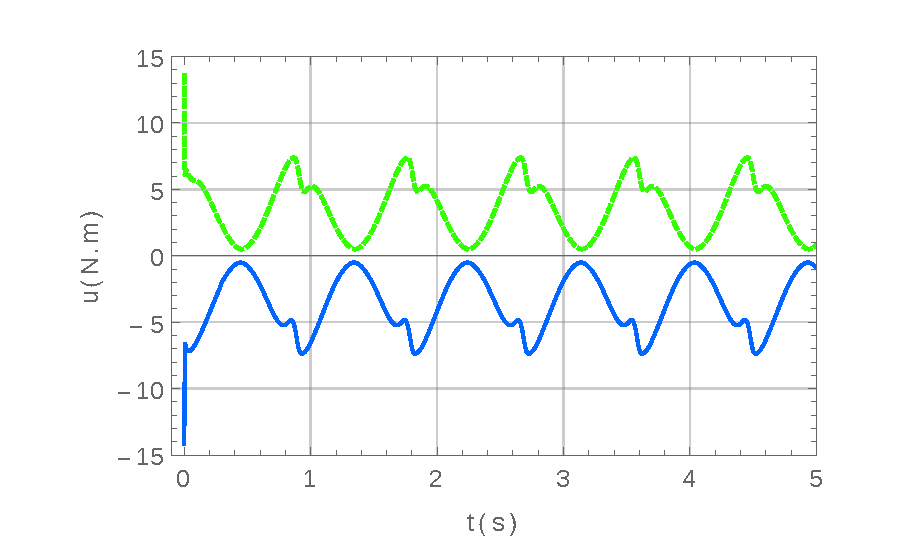
\includegraphics[scale=0.5]{ControlB2.pdf}
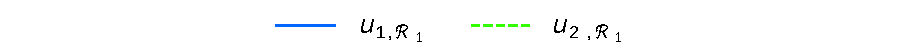
\includegraphics[scale=0.5]{ControlA1sub.pdf}
\label{fig:ControlB2}
\caption{Control inputs}
\end{minipage}
\end{figure}

Din\^amica do erro de controle:

\begin{figure}[H]
\centering
\subfigure[Position error norm]{%
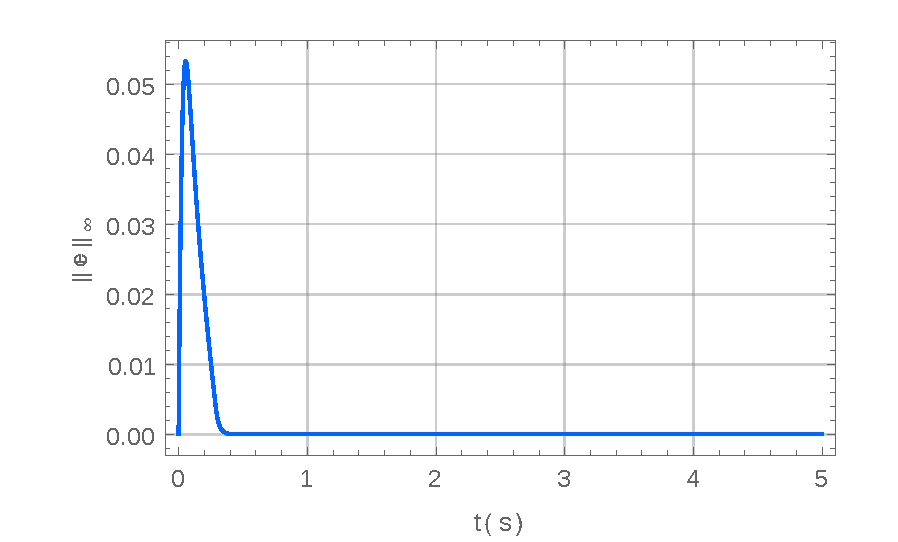
\includegraphics[scale=0.37]{PositionErrorB2.pdf}
\label{fig:PositionErrorB2}}
\quad
\subfigure[Velocity error norm]{%
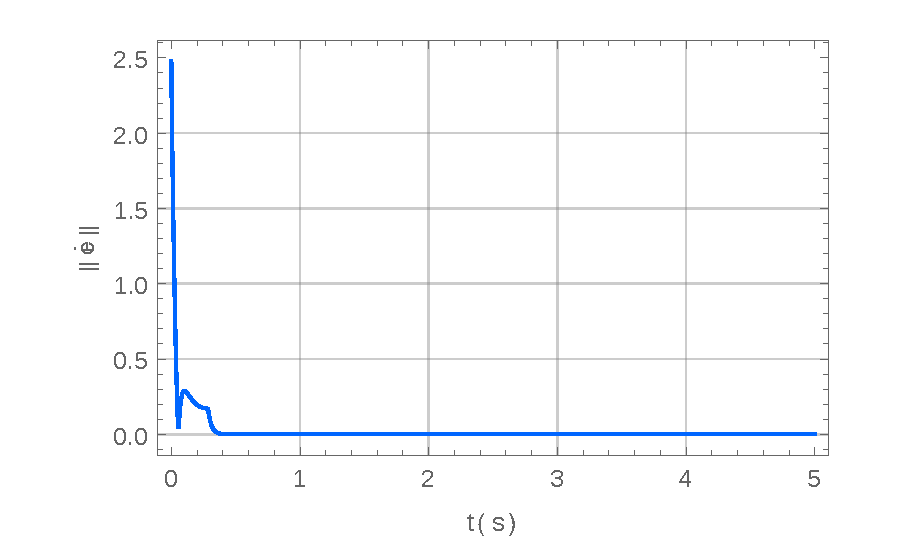
\includegraphics[scale=0.37]{VelocityErrorB2.pdf}
\label{fig:VelocityErrorB2}}
\subfigure[$||\ms|| = || \dot{\me} + \lambda \me ||$]{%
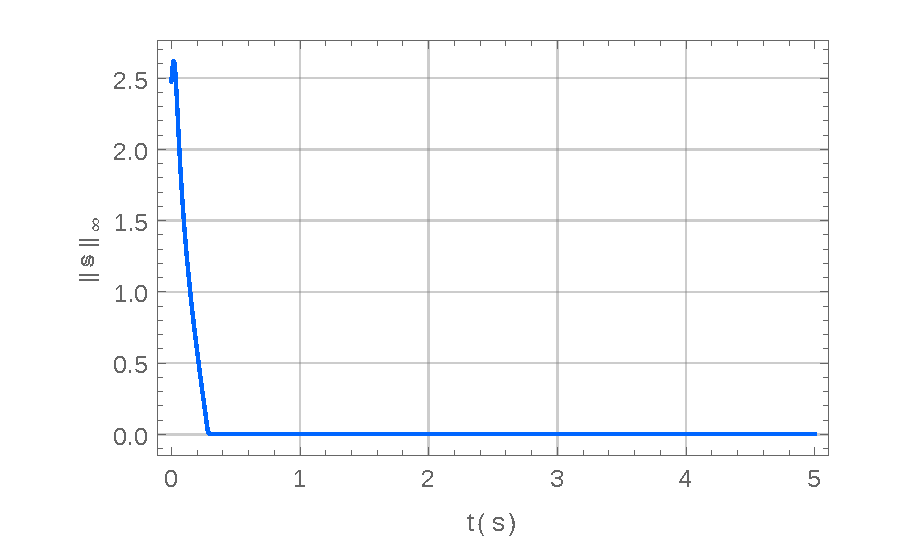
\includegraphics[scale=0.37]{sB2.pdf}
\label{fig:sB2}}
%
\caption{Error dynamics}
\label{fig:figure}
\end{figure}


\end{itemize}

Pode-se observar que, na maior parte do tempo, os esfor\c{c}os realizados pelos atuadores no caso do mecanismo desbalanceado s\~ao menores do que no caso do mecanismo balanceado. Esse resultado \'e esperado, pois a trajet\'oria de refer\^encia 2 \'e um movimento mais razoavelmente r\'apido, o que significa que a contrubui\c{c}\~ao do peso deve ser menos significativa do que a contribui\c{c}\~ao das for\c{c}as de in\'ercia nos esfor\c{c}os dos atuadores.

\end{itemize}